% Capítulo 2 – gerado a partir do relatório; edite livremente
\chapter{CARACTERIZAÇÃO DA PEÇA}

A Figura~\ref{fig:desenho} reproduz o desenho da peça. Do ponto de vista da usinagem, a engrenagem é formada por um aro dentado com diâmetro externo de 156 mm e largura de 48 mm, ligado ao cubo por uma alma de 14 mm de espessura. A alma é rebaixada nas duas faces até o diâmetro de 110 mm e tem quatro rasgos em arco, com extremidades de raio 9 mm, distribuídos sobre o diâmetro de 78 mm. O cubo tem diâmetro de 46 mm, sobressai 1,5 mm em relação às faces do aro (comprimento total de 51 mm) e termina em chanfro de 2 mm. O furo de Ø25 mm tem rasgo de chaveta de 8 mm, com 28,5 mm do fundo do rasgo à geratriz oposta do furo. A ligação da alma com o cubo e com o aro é feita com raios de 3 mm.


\begin{figure}[H]
\centering
\caption{Desenho da engrenagem e da cremalheira}\label{fig:desenho}
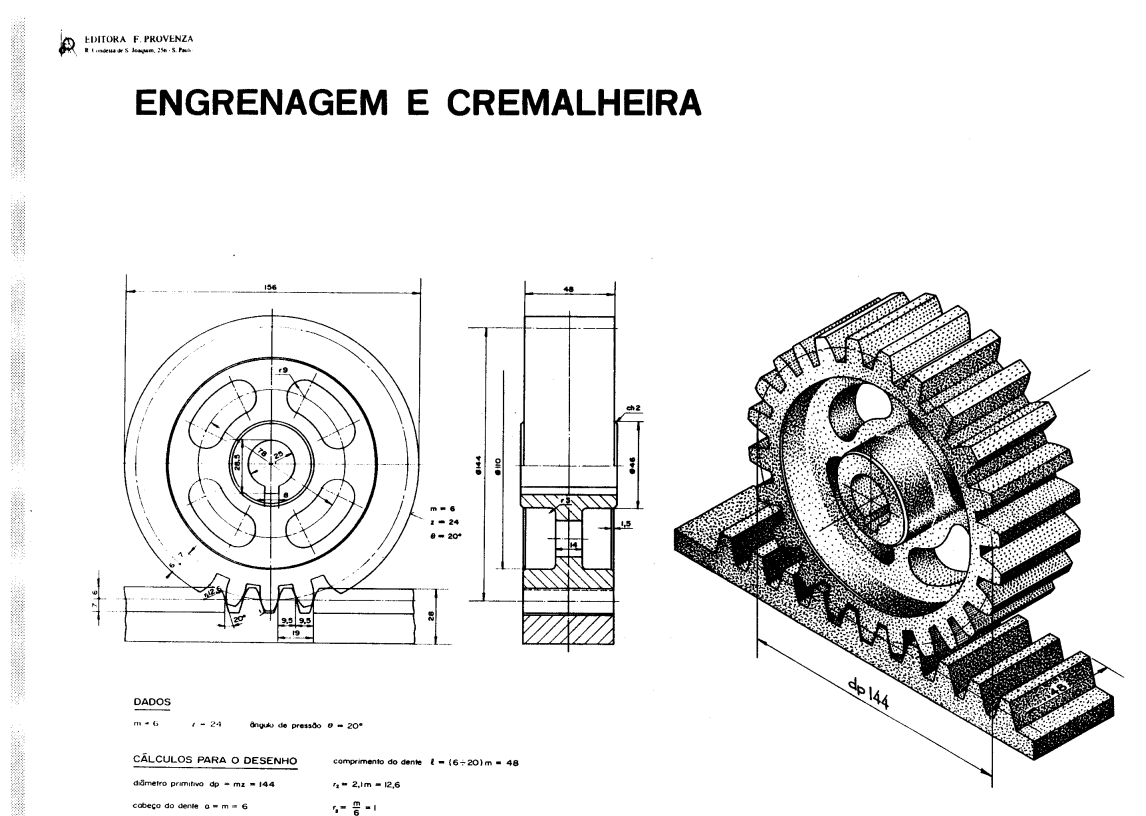
\includegraphics[width=15.5cm]{figuras/desenho_protec.png}
\fonte{Provenza (PROTEC).}
\end{figure}


\section{Material e especificações complementares}

O SAE 8620 é um aço baixa liga ao níquel-cromo-molibdênio, com cerca de 0,20 \% de carbono, próprio para cementação. Laminado e recozido, com dureza entre 170 e 200 HB, tem boa usinabilidade e corresponde ao grupo P2.1 dos catálogos de ferramentas (aço baixa liga recozido, 175 HB), que foi a referência para os dados de corte. Para o cálculo das forças foram usados os coeficientes de Kienzle do próprio 8620 apresentados em aula, K\textsubscript{s1} = 2100 N/mm² e 1 $-$ z = 0,74.


O desenho traz apenas as cotas nominais. Para planejar o acabamento das superfícies funcionais, foram adotadas as especificações do Quadro~\ref{quad:espec}, coerentes com a função da peça. São elas que justificam a retificação do furo e das faces do cubo depois do tratamento térmico.


\begin{quadro}[H]
\centering
\caption{Especificações adotadas para as superfícies funcionais}\label{quad:espec}
{\small\renewcommand{\arraystretch}{1.2}
\begin{tabular}{|>{\raggedright\arraybackslash}p{\dimexpr 0.1970\linewidth-2\tabcolsep\relax}|>{\raggedright\arraybackslash}p{\dimexpr 0.3878\linewidth-2\tabcolsep\relax}|>{\raggedright\arraybackslash}p{\dimexpr 0.4002\linewidth-2\tabcolsep\relax}|}
\hline
\rowcolor{cinza} \textbf{Superfície} & \textbf{Especificação adotada} & \textbf{Justificativa} \\ \hline
Furo Ø25 & H7; Ra 0,8 \textmu{}m & Montagem em eixo chavetado com ajuste H7/k6 \\ \hline
Faces do cubo & Comprimento 51,00 ± 0,02 mm; paralelismo e perpendicularidade ao furo de 0,02 mm; Ra 0,8 \textmu{}m & Encosto axial da engrenagem no eixo \\ \hline
Rasgo de chaveta & 8 JS9 & Chaveta paralela conforme DIN 6885 \\ \hline
Dentes & Qualidade 9 a 10 (DIN 3962); Ra 3,2 \textmu{}m & Transmissão pinhão-cremalheira em baixa velocidade \\ \hline
Tratamento térmico & Cementação, têmpera e revenimento; 58 a 62 HRC na superfície; camada de 0,8 a 1,0 mm & Resistência ao desgaste e à fadiga de contato dos flancos \\ \hline
Demais superfícies & ISO 2768-m; Ra 6,3 \textmu{}m & Superfícies sem função de montagem \\ \hline
\end{tabular}}
\fonte{Elaborado pelos autores.}
\end{quadro}


\section{Matéria-prima}

O bruto foi dimensionado com as tabelas de sobremetal mínimo vistas em aula (EM335, Aula 21), considerando o maior diâmetro da peça e o comprimento do cubo. Os valores adotados estão na Tabela~\ref{tab:sobremetal}. Nas faces e no furo, o sobremetal de retificação foi tomado um pouco acima do mínimo para absorver a distorção do tratamento térmico.


\begin{table}[H]
\centering
\caption{Sobremetais adotados e dimensões intermediárias}\label{tab:sobremetal}
{\small\renewcommand{\arraystretch}{1.2}
\begin{tabular}{|>{\raggedright\arraybackslash}p{\dimexpr 0.2373\linewidth-2\tabcolsep\relax}|>{\raggedright\arraybackslash}p{\dimexpr 0.3086\linewidth-2\tabcolsep\relax}|>{\centering\arraybackslash}p{\dimexpr 0.1899\linewidth-2\tabcolsep\relax}|>{\raggedright\arraybackslash}p{\dimexpr 0.2492\linewidth-2\tabcolsep\relax}|}
\hline
\rowcolor{cinza} \textbf{Superfície} & \textbf{Sobremetal mínimo (tabela)} & \textbf{Sobremetal adotado} & \textbf{Dimensão resultante} \\ \hline
Diâmetro externo Ø156 & 1,2 mm no raio (barras de Ø100 a Ø180) & 2,0 mm no raio & Barra de Ø160 \\ \hline
Faces (comprimento) & 3,0 mm por face (barras de Ø80 a Ø150) & 3,35 mm por face & Bruto com 58 mm \\ \hline
Faces do cubo (retificação plana) & 0,10 mm por face (faces até 100 mm) & 0,15 mm por face & Cubo torneado com 51,3 mm \\ \hline
Furo Ø25 (retificação interna, peça temperada) & 0,25 mm no raio (furo de Ø20 a Ø25, comprimento de 50 a 75 mm) & 0,25 mm no raio & Furo mandrilado em Ø24,5 \\ \hline
\end{tabular}}
\fonte{Elaborado pelos autores com base em EM335 – Aula 21 (Sobremetal de usinagem).}
\end{table}


O bruto é, portanto, um tarugo serrado de Ø160 $\times$ 58 mm, com massa de 9,2 kg. A peça pronta tem cerca de 3,4 kg, ou seja, aproximadamente 62 \% do material sai como cavaco, principalmente nos rebaixos da alma e nos vãos dos dentes. A Figura~\ref{fig:bruto} mostra a seção da peça torneada sobreposta ao bruto.


\begin{figure}[H]
\centering
\caption{Seção da peça torneada sobreposta ao bruto}\label{fig:bruto}
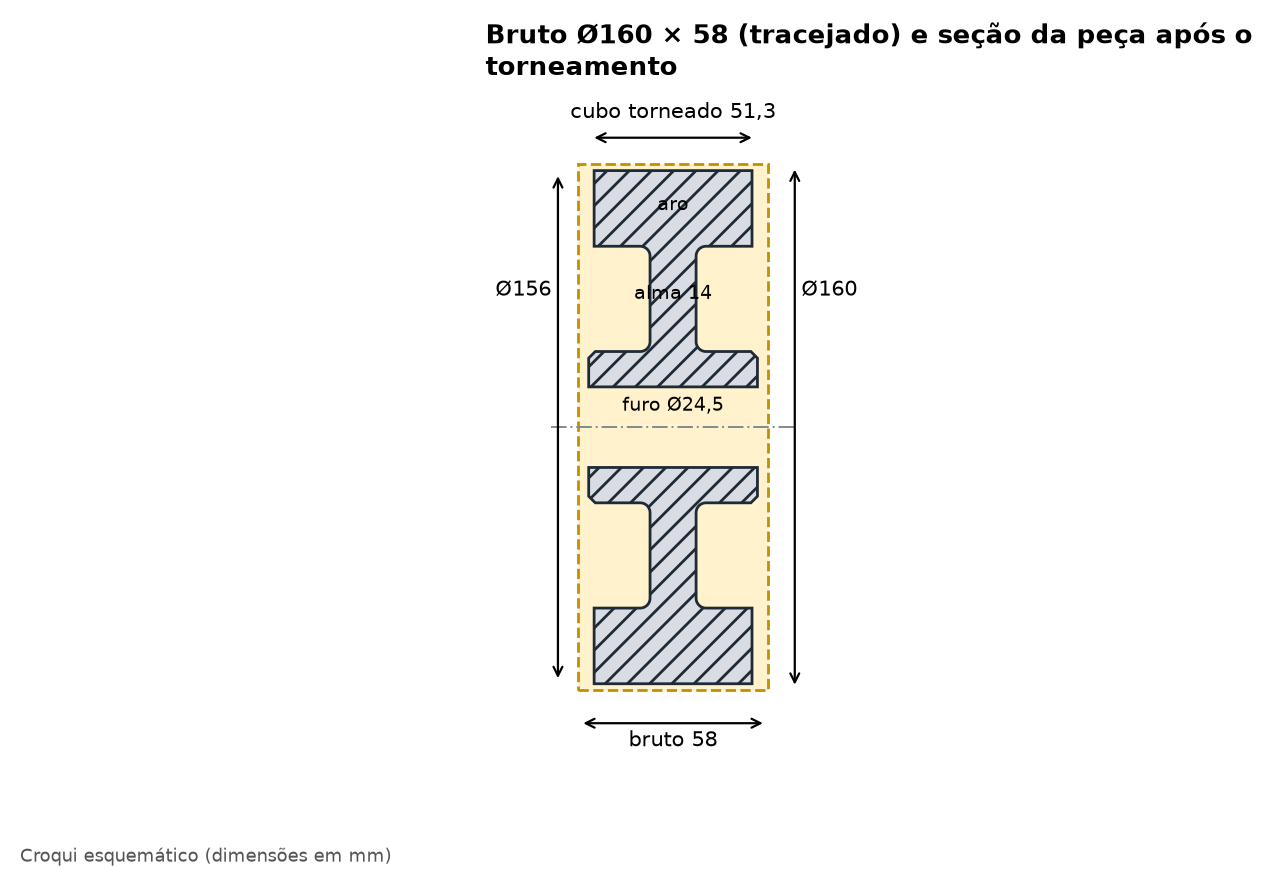
\includegraphics[width=10cm]{figuras/fig_bruto_peca.png}
\fonte{Elaborado pelos autores.}
\end{figure}

